\documentclass[aps,prl,superscriptaddress]{revtex4-1}
\usepackage{amsmath,amsfonts,amssymb}
\usepackage{graphicx}
\usepackage{comment}
\usepackage{subcaption}
\usepackage{hyperref}
\usepackage{braket}
\usepackage{CJK}

\newcommand{\midrule}{\hline}
\newcommand{\bottomrule}{\hline\hline}
\newcommand{\bs}{\boldsymbol}
\newcommand{\tr}{\text{tr}}

\usepackage{xcolor,framed}
\definecolor{shadecolor}{gray}{0.95}
% \verb|ax.plot(x,y)| for inline code
% \begin{shaded}\begin{verbatim} for block code
% \begin{subfigure}{0.48\textwidth} for subfigure

\graphicspath{{./figures/}}

% for including code snippets
\definecolor{lightblue}{rgb}{0.053,0.5,0.977}
\definecolor{deepblue}{rgb}{0,0,0.5}
\definecolor{deepred}{rgb}{0.6,0,0}
\definecolor{deepgreen}{rgb}{0,0.5,0}

\usepackage{listings}
\lstset{
language=python,
basicstyle=\footnotesize\scriptsize,
commentstyle=\color{lightblue}\ttfamily,
otherkeywords={\ as\ ,self},             % Add keywords here
keywordstyle=\color{deepblue}\ttfamily,
emph={MyClass,__init__},          % Custom highlighting
emphstyle=\color{deepred}\ttfamily,    % Custom highlighting style
stringstyle=\color{deepred},
frame=tb,                         % Any extra options here
showstringspaces=false            % 
}
\lstset{language=C++,
basicstyle=\ttfamily\scriptsize,
keywordstyle=\color{blue}\ttfamily,
stringstyle=\color{red}\ttfamily,
commentstyle=\color{gray}\ttfamily,
morecomment=[l][\color{magenta}]{\#},
}
\lstdefinestyle{Bash}{
language=Bash,
keywordstyle=\color{BlueViolet}\bfseries,
stringstyle=\color{Red},
showstringspaces=false,
basicstyle=\tiny\color{black},
numbers=none,
captionpos=b,
tabsize=4,
breaklines=true
}

\begin{document}
\begin{CJK*}{UTF8}{zhsong}
\title{Quantum Monte Carlo Compton profiles of solid and liquid lithium (Supplemental Materials)}
\author{Yubo Yang (杨煜波)}
\affiliation{Department of Physics, University of Illinois, Urbana, Illinois 61801, USA}
\author{Nozomu Hiraoka}
\affiliation{National Synchrotron Radiation Research Center, Hsinchu 30076, Taiwan}
\author{Kazuhiro Matsuda}
\affiliation{Graduate School of Science, Kyoto University, Kyoto 606-8502, Japan}
\author{Markus Holzmann}
\affiliation{Univ. Grenoble Alpes, CNRS, LPMMC, 38000 Grenoble, France}
\affiliation{Institut Laue Langevin, BP 156, F-38042 Grenoble Cedex 9, France}
\author{David M. Ceperley}
\affiliation{Department of Physics, University of Illinois, Urbana, Illinois 61801, USA}
\maketitle
\end{CJK*}

\subsection{Disordered Configurations}

Disordered configurations were generated from classical molecular dynamics (MD) simulations with the modified embedded atom potential (MEAM) as implemented in LAMMPS. 32 lithium configurations were generated in solid and liquid phases. The Li-Li structure factor was calculated from the MD runs and compared to X-ray data in Fig.~\ref{fig:lisk}.

\begin{figure}[h]
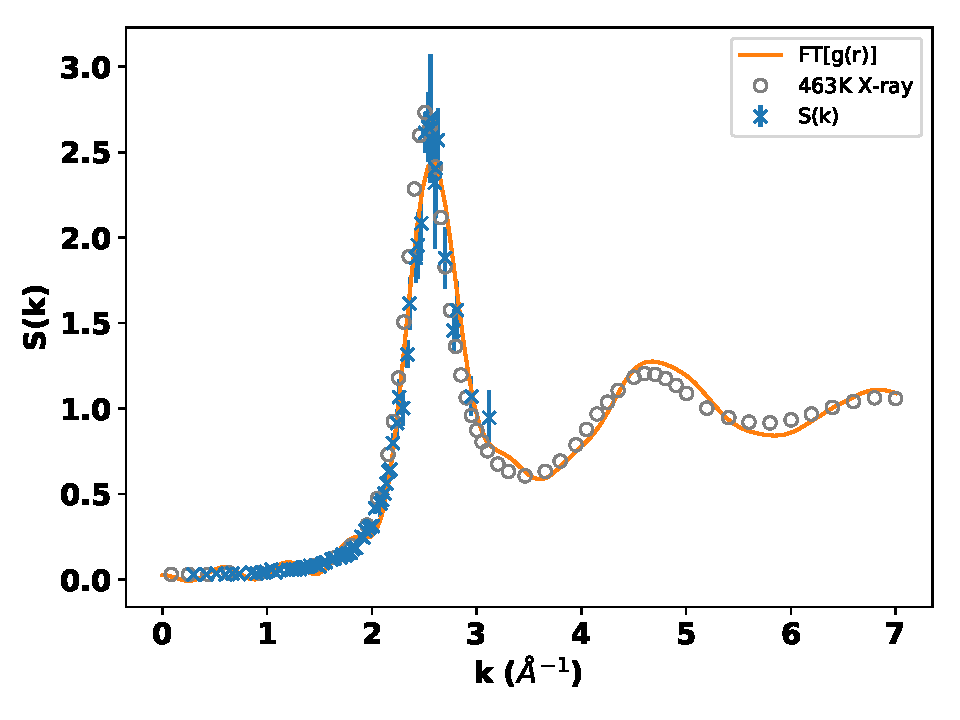
\includegraphics[scale=0.48]{009d_amass-cont1_t500}
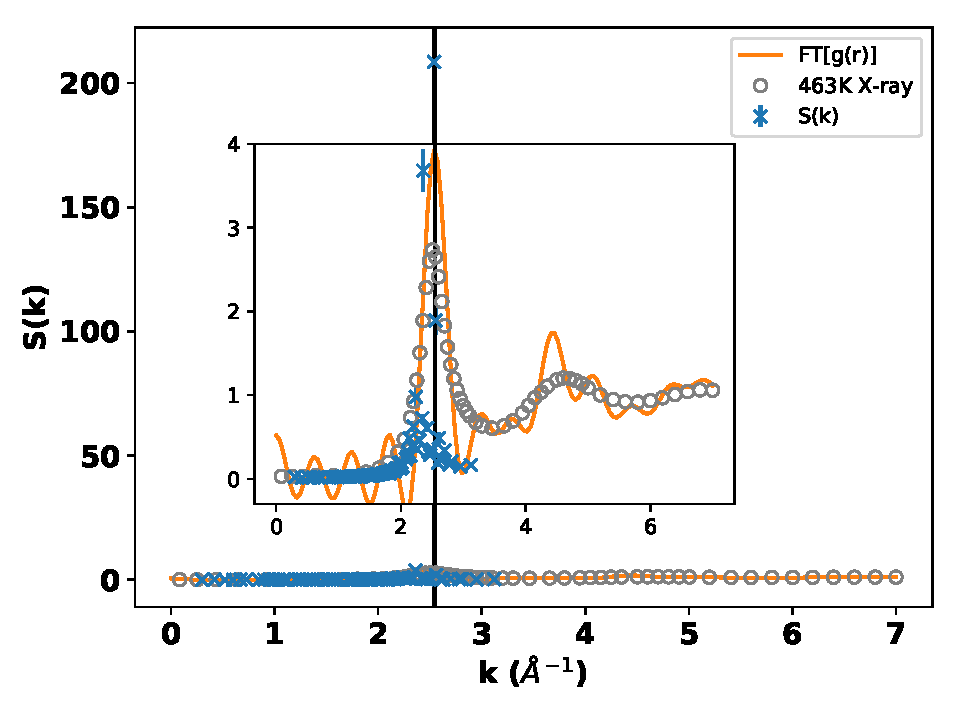
\includegraphics[scale=0.48]{009d_amass-temp330}
\caption{Structure factor of disordered lithium configurations in liquid (left) and solid (right) phases. 32 lithium configurations were generated in each phase. Each configuration contained 432 lithium atoms in a cubic box with side length 20.96$\AA$. The liquid configurations were generated at $T=500K$, whereas the solid configurations were generated at $T=330K$. The blue crosses are spherically-averaged $S(k)$ calculated directly in reciprocal space. The solid line is the Fourier transform of the real-space pair correlation function $g(r)$. The gray circles are experimental values from X-ray scattering~\cite{Waseda1981,Mokshin2018}.}
\label{fig:lisk}
\end{figure}

\subsection{QMC Energies}

The orbitals in the Slater determinant were obtained using KS-LDA. We used a planewave cutoff of 256 Ry in the all-electron calculation. The resultant orbitals were modified to remove the approximate electron-ion cusp, which is exactly re-introduced in the Jastrow. All pseudopotential calculations used the BFD pseudopotential and a planewave cutoff of 16 Ry.

QMC calculations were carried out at valence density $r_s=3.25$, consistent with the previous study~\cite{Filippi1999}. 
QMC energies of the all-electron simulations are shown in the first three rows of Table~\ref{tab:qmc-etv}. Timestep error is $\sim$ 0.1 mha/e/a.u.. Mix-estimator error of the kinetic energy is $\sim$ 4 mha/e. The mix-estimator errors are larger than their pseudopotential counterparts. Nevertheless, our DMC total energy of -2.5142 ha/e is within 1.5 mha/e of the -2.5129 ha/e obtained in a previous QMC study using localized basis and the PBE functional~\cite{Rasch2015}. The previous study was performed at a valence density of $r_s=3.24$, which is very close to our $r_s=3.25$.
Energies from the pseudopotential simulations are shown in the remaining rows of Table~\ref{tab:qmc-etv}. The difference between pseudopotential DMC and VMC total energies are consistently around 1 mha/e. Further, the timestep error is $\sim$ 0.1 mha/e/a.u. and the mix-estimator error of the kinetic energy is $<$ 1 mha/e. These small differences verify the high quality of our trial wavefunction for the valence electrons.

\begin{table}[h]
\caption{QMC energies and variance. All energies are reported in ha/e. Variance is in ha$^2$/e. Timestep is in ha$^{-1}$. Monte Carlo acceptance rate (acc) is in percent. Classical temperature is shown in Kelvin. $\langle\rangle$ indicates average over thermal ensemble and grand-canonical twist grid.}
\begin{tabular}{rrrllllll}
\toprule
 $N_e/N_{Li}$ &  Classical T &  $\langle N_e\rangle$ & method & timestep &    acc & $\langle E\rangle/\langle N_e\rangle$ & $\sigma_E^2/\langle N_e\rangle$ & $\langle T\rangle/\langle N_e\rangle$ \\
\midrule
            3 &            0 &                161.93 &    VMC &      0.8 &  43.51 &                           -2.51036(2) &                       0.0204(2) &                              2.506(2) \\
            3 &            0 &                161.93 &    DMC &     0.01 &  98.79 &                           -2.51413(1) &                      0.01888(2) &                             2.5097(4) \\
            3 &            0 &                161.93 &    DMC &    0.005 &  99.53 &                           -2.51416(1) &                      0.01890(2) &                             2.5098(3) \\
            1 &            0 &                 54.11 &    VMC &        2 &  81.88 &                           -0.25573(3) &                      0.00393(4) &                            0.15076(7) \\
            1 &            0 &                 54.11 &    DMC &      0.2 &   98.7 &                           -0.25709(1) &                      0.00432(2) &                            0.14974(3) \\
            1 &            0 &                 54.11 &    DMC &      0.1 &  99.47 &                          -0.256986(8) &                      0.00421(1) &                            0.14985(3) \\
            1 &            0 &                431.41 &    VMC &     3.25 &  71.64 &                          -0.254517(3) &                     0.004173(9) &                           0.150858(8) \\
            1 &            0 &                431.41 &    DMC &      0.2 &   98.7 &                          -0.255730(4) &                     0.004631(8) &                            0.15025(2) \\
            1 &            0 &                431.41 &    DMC &      0.1 &  99.47 &                          -0.255630(4) &                     0.004518(7) &                            0.15032(2) \\
            1 &          330 &                431.85 &    VMC &        3 &  73.91 &                        -0.2520480(10) &                     0.004274(3) &                           0.152858(3) \\
            1 &          330 &                431.85 &    DMC &      0.3 &  97.85 &                         -0.2534085(9) &                     0.004872(2) &                           0.152212(3) \\
            1 &          330 &                431.85 &    DMC &     0.15 &  99.11 &                         -0.2532710(9) &                     0.004803(2) &                           0.152279(3) \\
            1 &          500 &                431.90 &    VMC &        3 &  73.54 &                          -0.249699(1) &                     0.004383(3) &                           0.154636(3) \\
            1 &          500 &                431.90 &    DMC &      0.3 &  97.81 &                         -0.2511151(9) &                     0.005000(2) &                           0.154009(3) \\
            1 &          500 &                431.90 &    DMC &     0.15 &  99.09 &                         -0.2509826(9) &                     0.004937(2) &                           0.154079(3) \\
\bottomrule
\end{tabular}

\label{tab:qmc-etv}
\end{table}

\subsection{QMC Electronic Structure Factor}

The fluctuating electronic structure factor
\begin{align}
\delta S(k) \equiv \left\langle
(\rho_{\bs{k}}-\bar{\rho}_{\bs{k}})^* (\rho_{\bs{k}}-\bar{\rho}_{\bs{k}})
\right\rangle,
\end{align}
where $\rho_{\bs{k}} = \sum\limits_j^{N_e} e^{i\bs{r}_j\cdot\bs{k}}$ is the collective coordinate of the electrons. The $\braket{}$ denotes expectation value, and $\bar{\rho}_{\bs{k}}\equiv\braket{\rho}_{\bs{k}}$. The QMC fluctuating structure factors are shown in Fig.~\ref{fig:qmc-dsk}. All values are linearly extrapolated to remove the mix-estimator bias. The pseudopotential $\delta S(k)$ is insensitive to disorder. The $\delta S(k)$ from 432-atom simulations of perfect crystal, disordered solid, and liquid structures are indistinguishable from one another. Further, finite system size has only a small effect on the electronic structure factor, because the $\delta S(k)$ of the 54-atom simulation is very close to the 432-atom one. All pseudopotential $\delta S(k)$ can be accurately described by the RPA $S(k)$ at the same valence density when $k<0.4$ a.u.. Our all-electron structure factor agrees well with that from the previous QMC study~\cite{Rasch2015}.

\begin{figure}[h]
%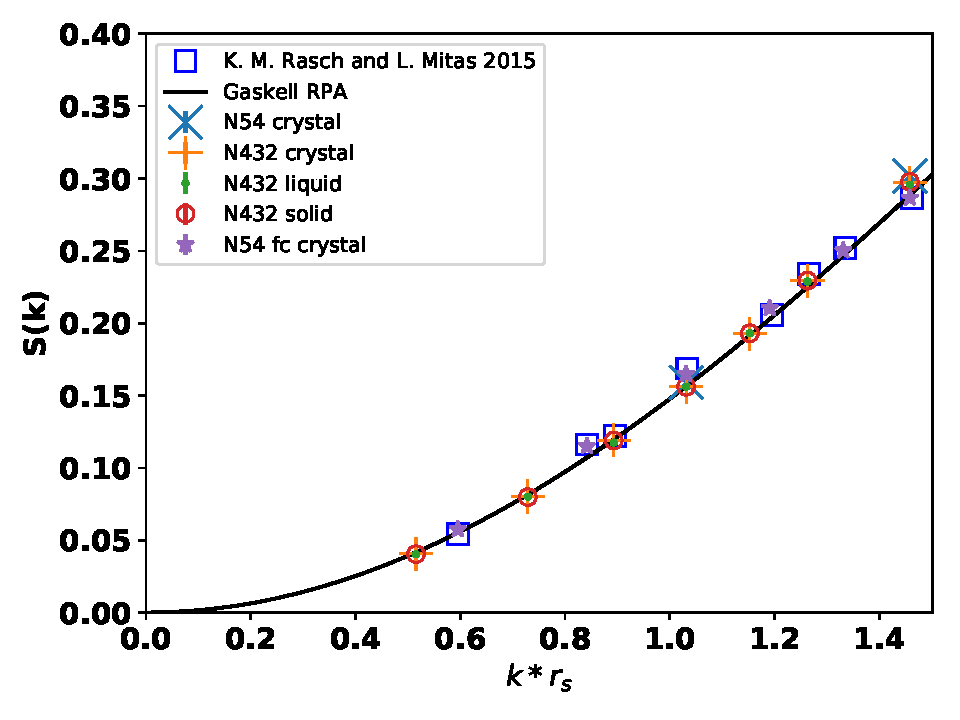
\includegraphics[scale=0.6]{li40bg_dsk-bfd-fc}
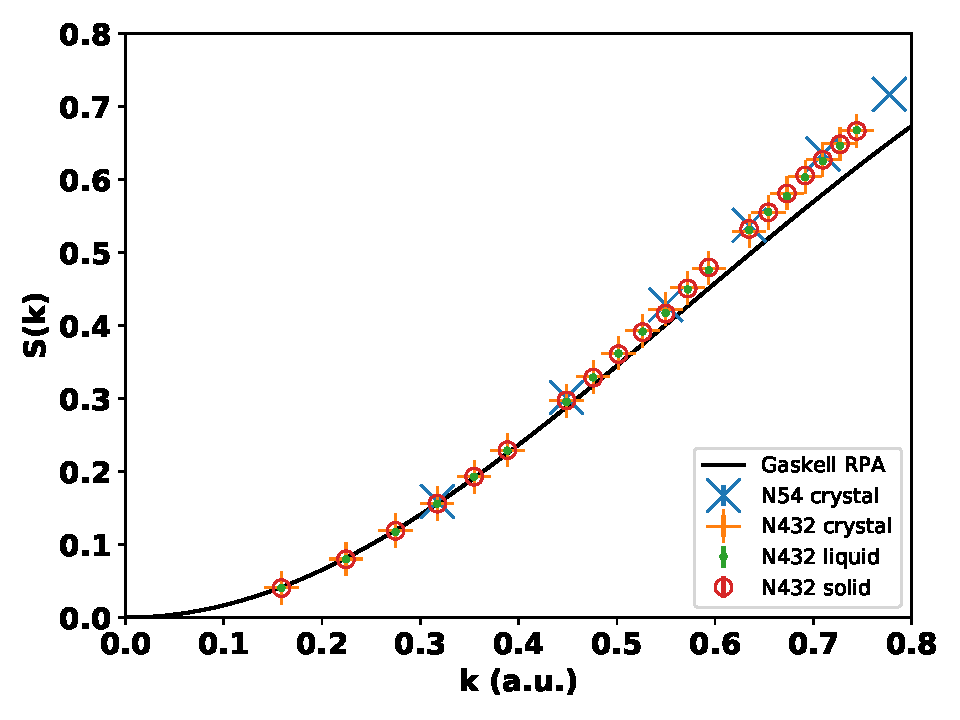
\includegraphics[width=0.48\linewidth]{li40bg_dsk-bfd}
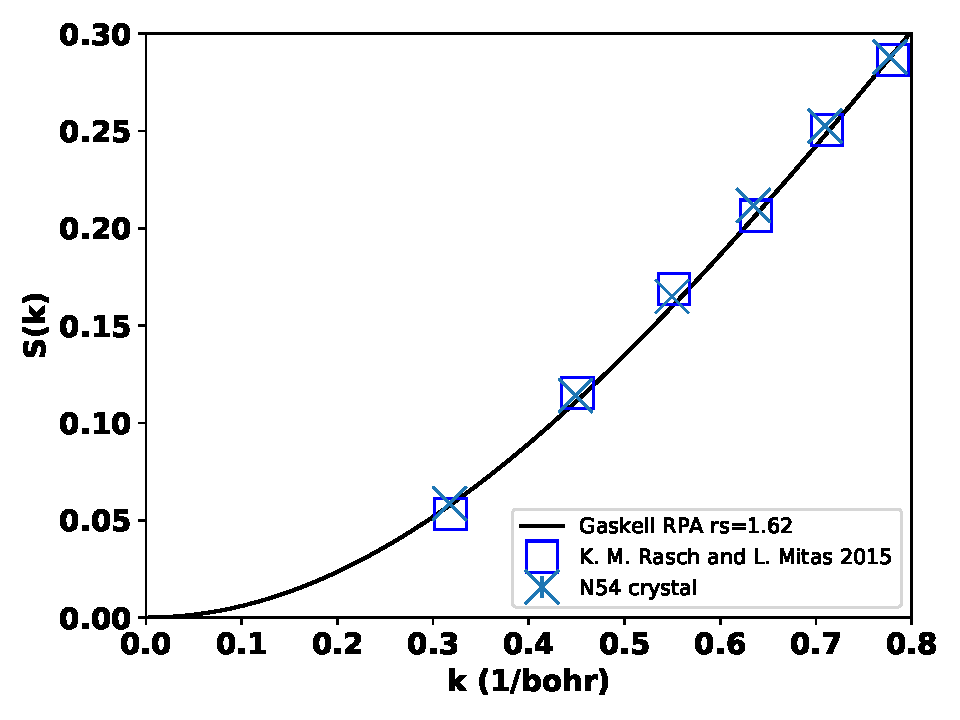
\includegraphics[width=0.48\linewidth]{li40bg_dsk-fc}
\caption{Electronic static structure factor of pseudopotential (left) and all-electron (right) QMC simulations in 54-atom and 432-atom simulation cells. The black line in the left plot is RPA $S(k)$ at valence density $r_s=3.25$. It fits lithium valence $S(k)$ remarkably well for $k<0.4$ bohr$^{-1}$. In the right plot, the black line is RPA $S(k)$ at density $r_s=3.25/\sqrt{3}$. \label{fig:qmc-dsk}}
\end{figure}


\subsection{QMC Momentum Distribution}

The momentum distribution is obtained on a cubic regular grid with spacing $dk=0.040$ a.u. in reciprocal space. To achieve this grid spacing, uniform twist-average grids of size $8^3$ and $4^3$ are used in the 54-atom and 432-atom simulations, respectively. The twist-average grid is $\Gamma$-centered in the perfect crystal calculations and shifted by $dk/2$ in all directions in disordered calculations. In the perfect crystal, cubic symmetries reduce the number of unique twists from 64 to 4 and 512 to 20 on a shifted grid, and 64 to 10 and 512 to 35 on a $\Gamma$-centered grid. The reciprocal-space grid is truncated at a spherical cutoff of $1.49$ a.u. in the solid and liquid simulations.
%The tail of the momentum distribution is extended to at least $3.0$ a.u. in post-processing.
%in 1/48th of the cubic reciprocal space, representing the irreducible wedge. The results are unfolded using cubic symmetries onto a regular grid with a spherical cutoff.

\begin{figure}[h]
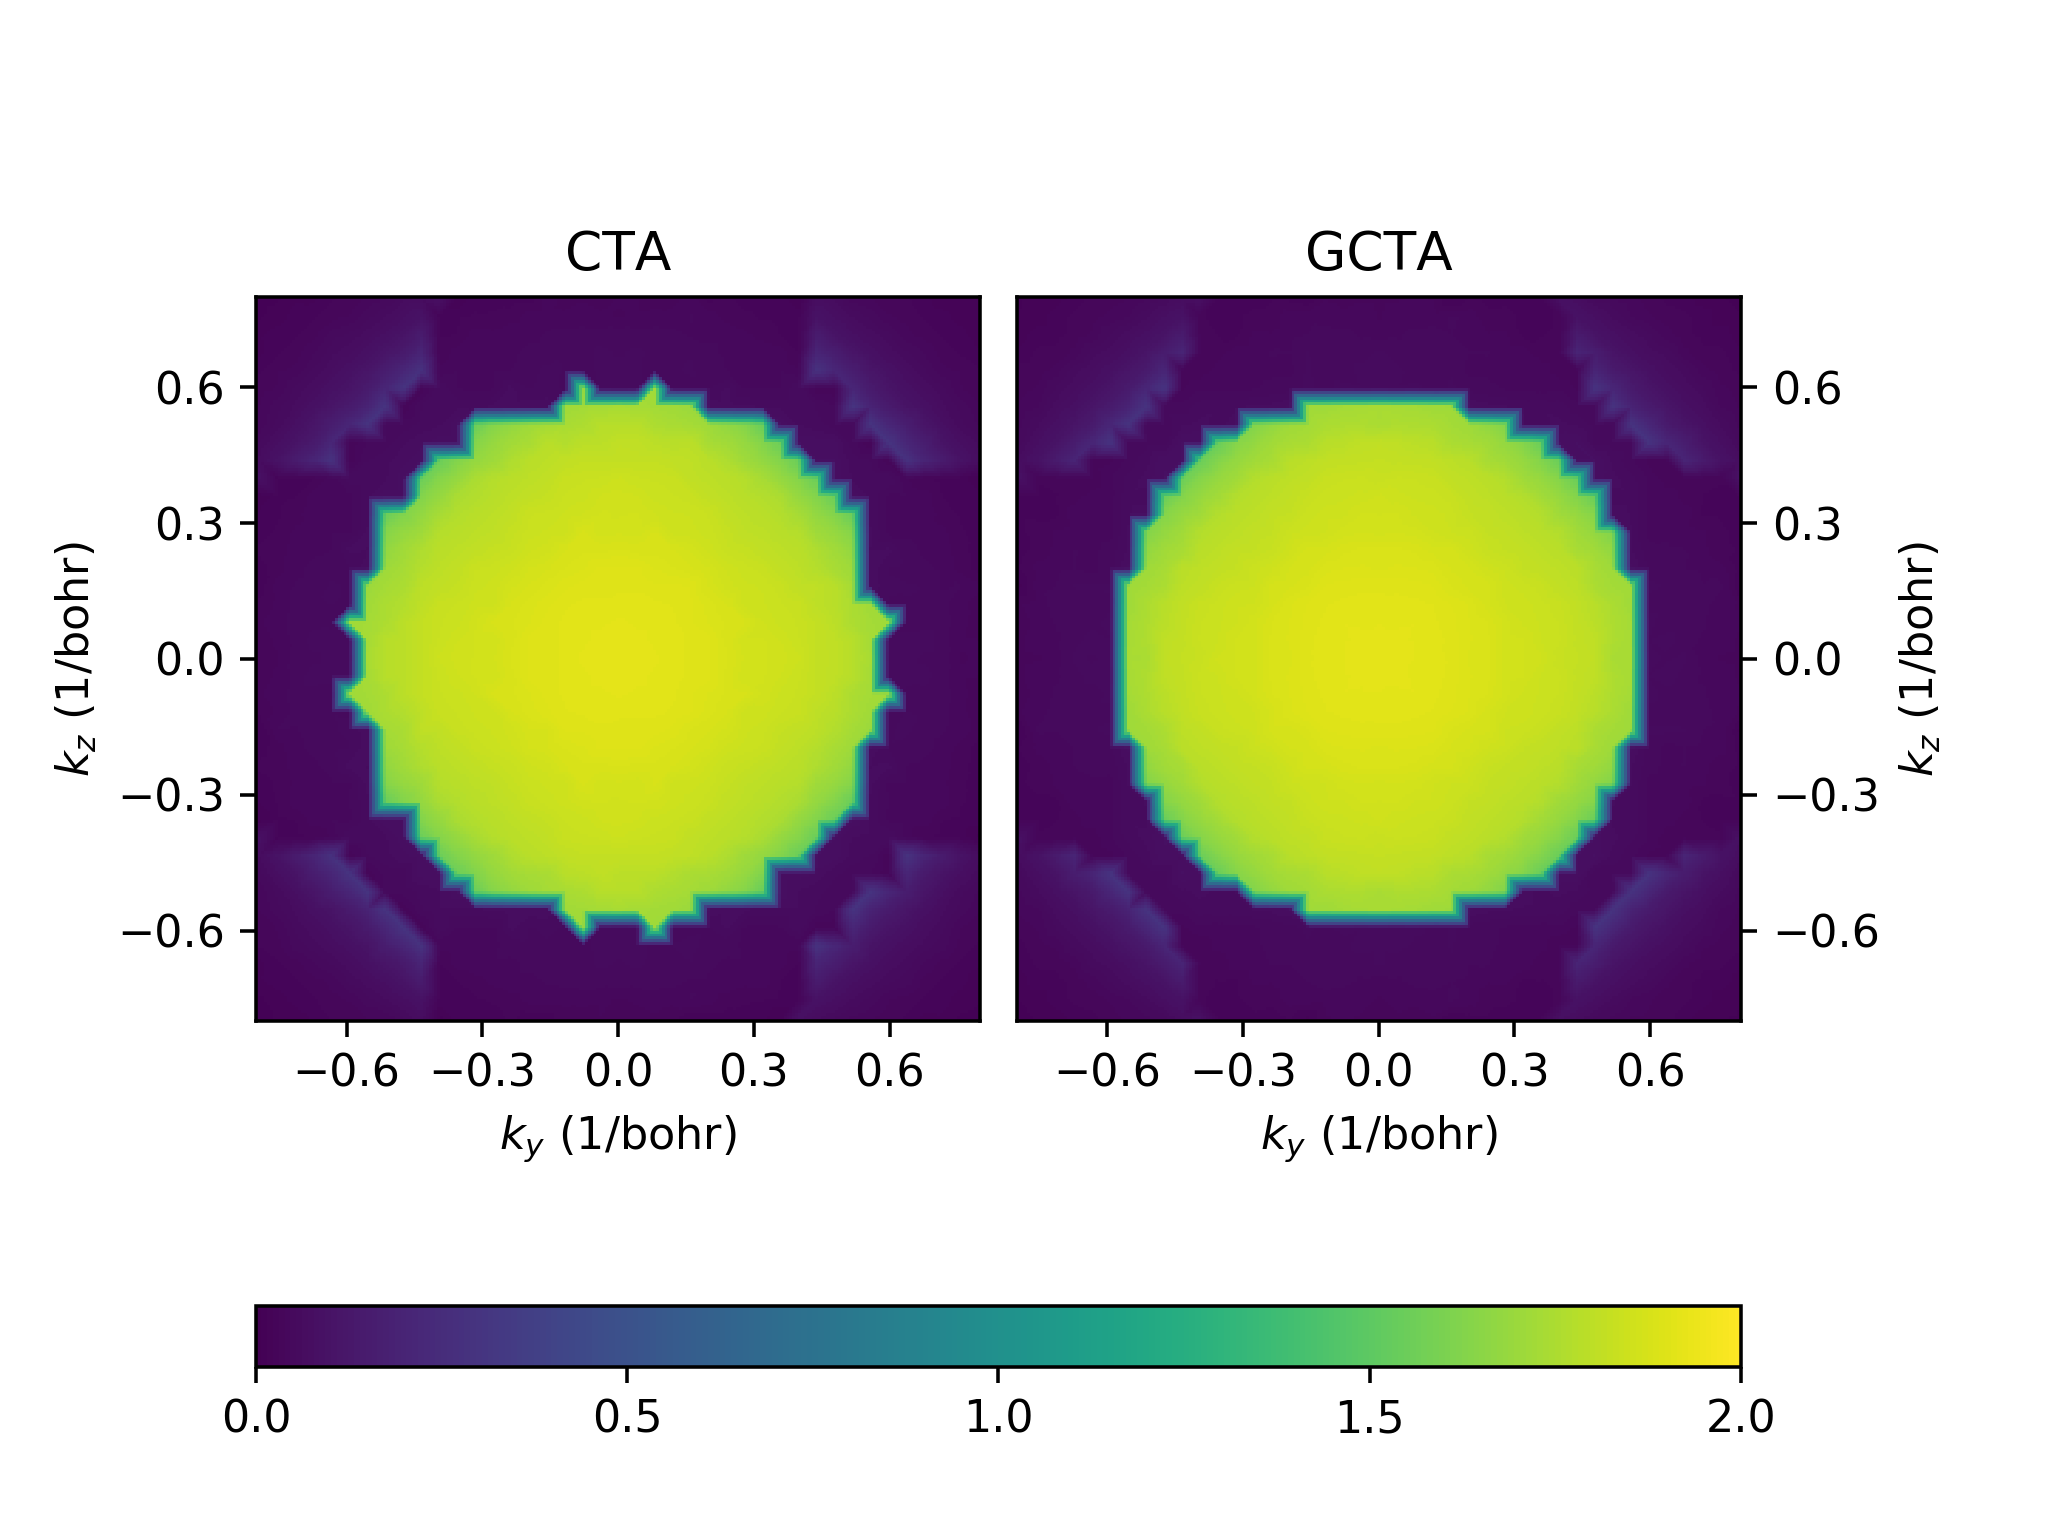
\includegraphics[width=0.8\linewidth]{li53_anofk-n54-ta-nk2d}
\caption{[100] slice of n($\bs{k}$) at $k_x=0$ from canonical twist average grid (CTA) and grand-canonical twist average grid (GCTA). Occupation outside the Fermi surface can be seen as small extrusions along $k_y$ or $k_z$ in the canonical case. Both the main and secondary Fermi surfaces are visibly more circular in the grand-canonical case.}
\end{figure}

A QMC Compton profile is computed in four steps. First, the 3D DMC $n(\bs{k})$ is linearly extrapolated to reduce the mix-estimator bias using VMC data. Second, the linearly-extrapolated $n(\bs{k})$ is spherically averaged to obtain a 1D distribution $n(k)$. Third, the 1D $n(k)$ is extended to large k using a model function eqn.~(\ref{eq:nktail}), which is inspired by the momentum distribution of hydrogen-like atoms
\begin{align} \label{eq:nktail}
n_{tail}(k, A, Z) = 2A\left(\dfrac{2Z}{(k^2+Z^2)^2}\right)^2,
\end{align}
where the $A$ and $Z$ are parameters are chosen to satisfy the sum rules as shown in Table~\ref{tab:crystal-ntsum}. Fourth and finally, the 1D $n(k)$ is integrated to obtain the spherically-averaged Compton profile $J(p)$ via eqn.~(\ref{eq:jp1d}) and split into two parts at a cutoff momentum $k_c$
\begin{align} \label{eq:jp1d}
J(p) = \left( \dfrac{(2\pi)^3}{\Omega/N_{Li}} \right)^{-1} \left[
\int\limits_p^{k_c} k n(k) dk + \int\limits_{k_c}^{\infty} k n_{tail}(k, A^*, Z^*) dk
\right],
\end{align}
where $\Omega$ is the volume of the supercell, $N_{Li}$ is the number of lithium atoms in the supercell, and $A^*$, $Z^*$ are chosen to satisfy momentum distribution sum rules. %The prefactor is needed because $n(\bs{k})$ in simulation is scaled by reciprocal volume and is always in the range [0, 2].
The sum-rules of the momentum distribution and the Compton profile in our convention are
\begin{align}
\left( \dfrac{(2\pi)^3}{\Omega/N_{Li}} \right)^{-1} \int d\bs{k} n(\bs{k}) =& \braket{N_e}/N_{Li}\equiv \bar{N}, \label{eq:nsum} \\
\left( \dfrac{(2\pi)^3}{\Omega/N_{Li}} \right)^{-1} \int d\bs{k} n(\bs{k})~\frac{\hbar^2k^2}{2m_e} =& \braket{T}/N_{Li} \equiv \bar{T}, \label{eq:tsum} \\
\int_{-\infty}^{\infty} dp J(p) =& \braket{N_e}/N_{Li}, \label{eq:jpsum}
\end{align}
where $\braket{T}$ is the expectation value of the total kinetic energy.
The fitted values in the tail function eqn.~(\ref{eq:nktail}) are shown in Tables~\ref{tab:crystal-ntsum}, along with sum-rule compliance.

\begin{table}[h]
\caption{Fits to $n(k)$ tails and sum rule compliance. $\bar{N}$ and $\bar{T}$ are the normalization and kinetic energy sum rules as defined in eqn.~(\ref{eq:nsum}) an (\ref{eq:tsum}). $\bar{N}_0$ and $\bar{T}_0$ are expected sum-rule values calculated from Table~\ref{tab:qmc-etv}. All sum-rule integrals are split into two parts at $k=k_c$ in the same way as eq.~(\ref{eq:jp1d}). $\Delta n(k_c)\equiv n_{tail}(k_c)-n(k_c)$ is the difference between the fit analytical tail and QMC data at the split point. The second row is ``full-core valence'' obtained by subtracting the HF core contribution from the QMC ae calculation. The HF core kinetic energy of the Li atom is 7.2239067 ha.}
\begin{tabular}{rrrlrrrrrrrr}
\toprule
 $N_e/N_{Li}$ &  Classical T &  $N_{Li}$ &    $\bar{T}_0$ &  $\bar{T}$ &  $\bar{N}_0$ &  $\bar{N}$ &       A &       Z &  $k_c$ &  $\Delta n(k_c)$ &  $n(k_c)$ \\
\midrule
            3 &            0 &        54 &       7.539(2) &     7.5388 &       2.9986 &     2.9986 &  7.1015 &  2.7625 &   1.50 &          -0.0064 &    0.0519 \\
            3 &            0 &        54 &       0.315(2) &     0.3149 &       0.9986 &     0.9986 &  0.1831 &  2.9175 &   1.50 &          -0.0013 &    0.0023 \\
            1 &            0 &        54 &     0.14925(7) &     0.1488 &       1.0021 &     1.0030 &  0.0213 &  0.4958 &   1.45 &           0.0008 &    0.0006 \\
            1 &            0 &       432 &     0.14958(4) &     0.1494 &       0.9986 &     0.9989 &  0.0220 &  0.4959 &   1.45 &           0.0005 &    0.0009 \\
            1 &          330 &       432 &    0.151647(7) &     0.1519 &       0.9996 &     0.9992 &  0.0236 &  0.4961 &   1.45 &           0.0003 &    0.0013 \\
            1 &          500 &       432 &    0.153489(8) &     0.1539 &       0.9998 &     0.9990 &  0.0258 &  0.4964 &   1.45 &           0.0001 &    0.0015 \\
\bottomrule
\end{tabular}

\label{tab:crystal-ntsum}
\end{table}

Tail models in Table~\ref{tab:crystal-ntsum} are shown along with QMC $n(k)$ data in Fig.~\ref{fig:qmc-tail-model}. The QMC all-electron $n(k)$ for the crystal appears to decay slightly slower than HF core $n(k)$ at large $k$. This causes the full-core valence momentum distribution to have a much longer tail than the pseudopotential ones.

\begin{figure}[h]
\begin{minipage}{0.49\linewidth}
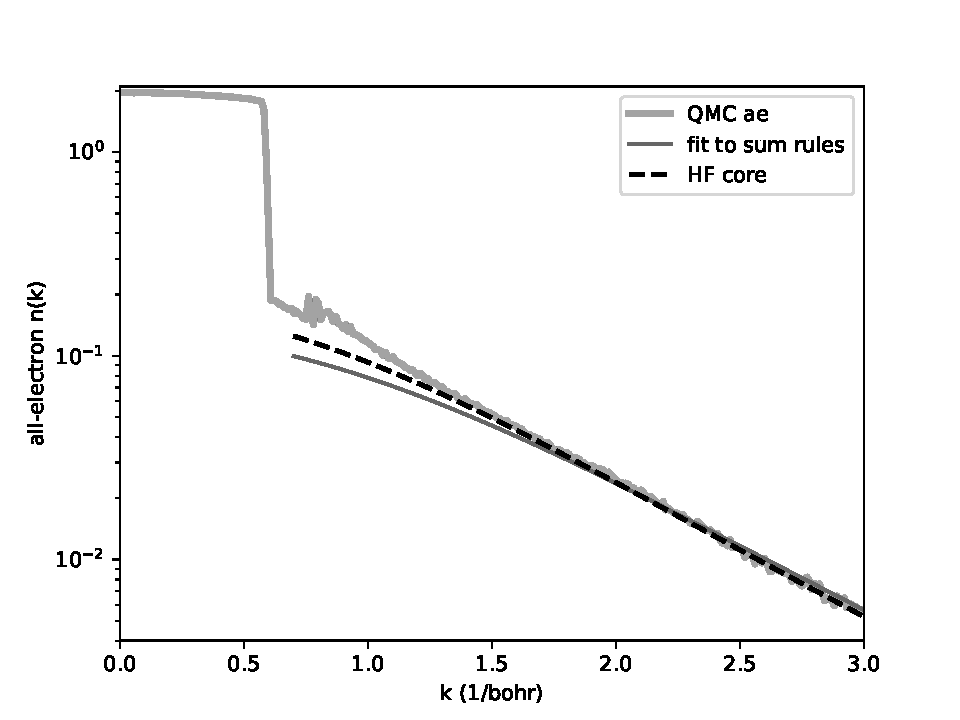
\includegraphics[width=\columnwidth]{li62e_ae-hf-tail}
(a) all-electron $n(k)$
\end{minipage}
\begin{minipage}{0.49\linewidth}
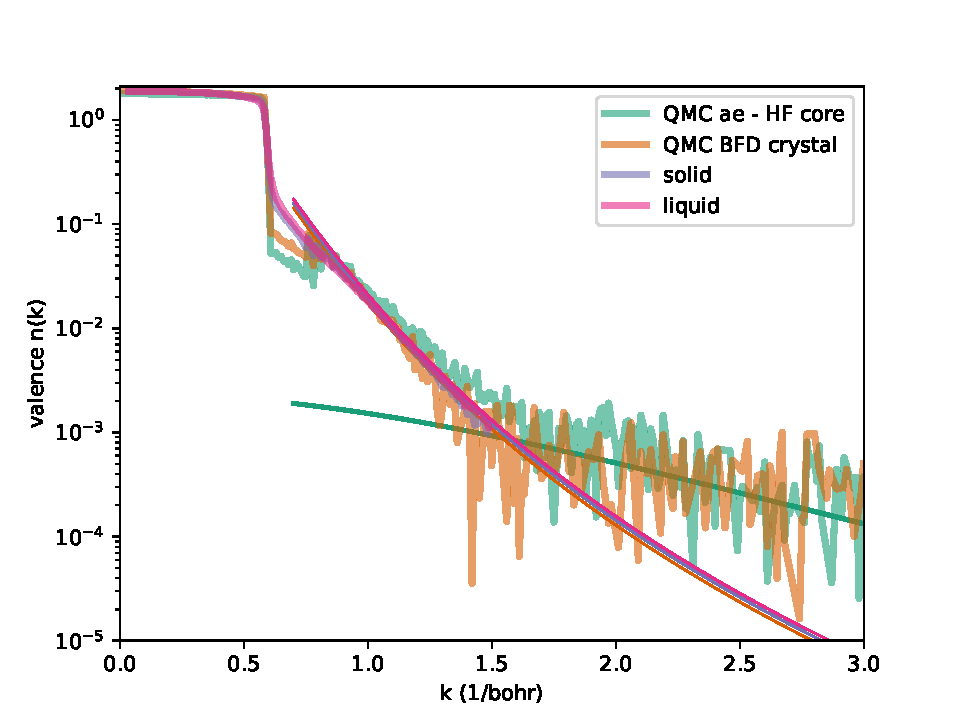
\includegraphics[width=\columnwidth]{li62e_valence-tail}
(b) valence $n(k)$
\end{minipage}
\caption{Models of the high-momentum tail of $n(k)$ based on sum-rule compliance. Left plot shows all-electron momentum distribution from QMC (thick gray line) and Li atomic core contribution from HF (dashed black line). The thin gray line is the $n(k)$ tail model for QMC. Right plot shows valence momentum distributions from QMC (thick colored lines). Each thin line is the tail model for the QMC $n(k)$ of corresponding color. The statistical error of QMC $n(k)$ is on the order of $10^{-4}$ for $k>1.5$, so data close to $10^{-4}$ at large $k$ are not reliable.}
\label{fig:qmc-tail-model}
\end{figure}

\bibliographystyle{apsrev4-1}
\bibliography{ref}

\end{document}
